\subsubsection*{January 7, 2020}
\section*{Course Overview}
\begin{itemize}
	\item Abstract algebra: groups, rings, fields.
	\item Number Theory, arbitrary precision integer arithmetics. 
	\item Cryptographic algorithms
\end{itemize}
\section{Groups}
We first define the group, which we will be using extensively. 
\begin{defn}{Group}
	A \ul{group} is a set $G$ with a binary operation ``$\circ$'' such that
	\begin{itemize}
		\item $G$ is closed under $\circ$.
		\item $G$ is associative. 
		\item There is an Identity Element: $\exists e\in G \mid x\circ e = e\circ x = x \ \forall x\in G$. 
		\item Inverses: $\forall x \in G\ \exists y\in G\mid x\circ y = y \circ x = e$. 
	\end{itemize}
\end{defn}

\begin{defn}{Abelian Group}
If $\circ$ is commutative in group $G$, we call $G$ \ul{Abelian}. In that case, $G$ is often written additively; i.e. we use ``$+$'' for ``$\circ$''.

(If $\circ$ is not commutative, we often write $G$ multiplicatively.)	
\end{defn}

\begin{defn}{Subgroup}
Let $G$ be a group, and $\emptyset\neq H \subseteq G$. Then $H$ is called a \ul{subgroup} of $G$ if $H$ is also a group. 
\end{defn}

A small proof to begin\dots 
\begin{proposition}
Let $G$ be a group and $x\in G$. Then $x$ has a unique inverse $y$, so we can write $y=x^{-1}$. 
\end{proposition}
\begin{proof}
Assume $y$ and $z$ are both inverses of $x$. 
\begin{align*}
y &= y \circ (x\circ z) = (y\circ x) \circ z = z	
\end{align*}
\end{proof}

\begin{proposition}
A non-empty subset $H\subseteq G$ is a subgroup of $G$ iff $xy^{-1}\in H\ \forall x, y\in H$. 
\end{proposition}
\begin{proof}
($\Rightarrow$) 
\begin{itemize}
	\item Identity: Pick $x\in H$. Then $xx^{-1}=e\in H$. 
	\item Inverse: If $y\in H$, $ey^{-1}=y^{-1}\in H$
	\item Closure: If $x, y\in H$, $y^{-1}\in H$, so $x(y^{-1})^{-1}=xy\in H$. 
\end{itemize}

($\Leftarrow$) If $H$ is a group, then $y^{-1}\in H$ (existence of unverse) and $xy^{-1}\in H$ (closure of $\circ$). 
\end{proof}

\example
\begin{itemize}
\item Every vector space (without the scalars) is an Abelian group with identity $\vec{0}$. 
\item Modular arithmetic: 
\[\Z_n = \{0, 1, 2, \dots, n-1\}\]

$\Z_n$ is an Abelian group under modular addition. 
\[\Z_n^*=\{k\in \Z_n\mid gcd(k, n) = 1\}\]
$\Z_n^*$ is an Abelian group under modular multiplication (this is sometimes also $\mathbb{U}_n$).

Let's take $\Z_4 - \{0\}$ and why it's not a group under multiplication. We can create a multiplication table: 
\begin{center}
\begin{tabular}{c|ccc}
$\circ$ & $1$ & $2$ & $3$ \\ \hline
$1$     & $1$ & $2$ & $3$ \\
$2$     & $2$ & $0$ & $2$ \\
$3$     & $3$ & $2$ & $1$
\end{tabular}
\end{center}

However there is no such problem with $\Z_4^*$: 
\begin{center}
\begin{tabular}{c|cc}
$\circ$ & $1$ & $3$ \\ \hline
$1$     & $1$ & $3$ \\
$3$     & $3$ & $1$
\end{tabular}
\end{center}
\end{itemize}

\begin{defn}{Cyclic}
	A group $G$ is called \ul{cyclic} if $\exists g\in G$ (called generator) such that $G = \{g^n\mid n\in \Z\}$. 
\end{defn}
\example
$Z_n$ are cyclic grous with generator 1. 

$\Z_4^*$ is cyclic with generator $3$. 

\example The Klein $4$-group is not cyclic: 
\[K = \{(0,0), (1,0), (0,1), (1,1)\}\]
with componentwise addition mod $2$. 
\[K = \Z_2\oplus \Z_2 = \{(k,l)\mid k\in \Z_2, l\in \Z_2\}\]

\begin{proposition}
Every cyclic group is Abelian. 	
\end{proposition}
\begin{proof}
Let $x, y\in G$, a cyclic Abelian group. Let $g$ be the generator in $G$. We write $x = g^a$ and $y = g^b$. Then $\displaystyle xy = g^ag^b = \underbrace{g\circ g\circ \cdots \circ g}_{\text{$k+l$ times}} = g^bg^a = yx$. 
\end{proof}

\example
The symmetry transformation of an equilateral $\triangle$ form a group under composition. 
\[D_3 = \{id, 120^\circ, 240^\circ, top, left, right\}\]
\\
\begin{center}
\begin{tikzpicture}
	\coordinate[label=above:$A$](a) at (0, 0.73205);
	\coordinate[label=below:$B$](b) at (-1,-1);
	\coordinate[label=below:$C$](c) at (1,-1);
	\draw (a) -- (b) -- (c) -- cycle;
	\draw[->,>=stealth',semithick] (-30:2) arc[radius=2.7, start angle=0, end angle=60] node[midway, xshift=15] {$120^\circ$};
	\draw[->,>=stealth',semithick] (2.4,-1) arc[radius=2.4, start angle=-20, end angle=200] node[midway, yshift=10] {$240^\circ$};
\end{tikzpicture}
\qquad
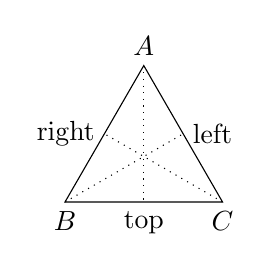
\begin{tikzpicture}
	\coordinate[label=above:$A$](a) at (0, 0.73205);
	\coordinate[label=below:$B$](b) at (-1,-1);
	\coordinate[label=below:$C$](c) at (1,-1);
	\draw (a) -- (b) -- (c) -- cycle;
	\draw[dotted] (a) -- (0,-1) node[below] {top};
	\draw[dotted] (b) -- (0.5,-0.133975) node[right] {left};
	\draw[dotted] (c) -- (-0.5,-0.133975) node[left] {right};
\end{tikzpicture}
\vspace{2em}

\begin{tabular}{c|cccccc}
$\circ$     & id          & $120^\circ$ & $240^\circ$ & top         & left        & right       \\ \hline
id          & id          & $120^\circ$ & $240^\circ$ & top         & left        & right       \\
$120^\circ$ & $120^\circ$ & $240^\circ$ & id          & left        & right       & top         \\
$240^\circ$ & $240^\circ$ & id          & $120^\circ$ & right       & top         & left        \\
top         & top         & right       & left        & id          & $240^\circ$ & $120^\circ$ \\
left        & left        & top         & right       & $120^\circ$ & id          & $240^\circ$ \\
right       & right       & left        & top         & $240^\circ$ & $120^\circ$ & id         
\end{tabular}
\end{center}


\begin{defn}{Equivalence}
Let $G$ be a group and $H$ a subgroup. Define the relation $x \sim y$ if $xy^{-1}\in H$. 
\end{defn}
\begin{proposition}
$\sim$ is an equivalence relation on $G$. 	\end{proposition}

If $H = \{e\}$, then $\sim$ is $=$. 

If $H = G$, then $\sim$ is trivial. 

\begin{proof}
We need to show that $\sim$ is
\begin{itemize}	
\item reflexive: $x\sim x$ for all $x\in G$
\[xx^{-1}=e\in H.\]
\item symmetric: $x\sim y \iff y\sim x$ for all $x, y\in G$

Suppose $x\sim y$. Then $xy^{-1}\in H$. So $(xy^{-1})^{-1}=yx^{-1}\in H\implies y\sim x$. 
\item transitive: If $x\sim y, y\sim z$ then $x\sim z$ for all $x, y, z \in G$. 

Suppose $x\sim y, y\sim z$. Then $xy^{-1}\in H, yz^{-1}\in H$. Then $(xy^{-1})(yz^{-1})=x(y^{-1}y)z^{-1}=xz^{-1}\in H\implies x\sim z$. 
\end{itemize}
\end{proof}

If $\sim$ is an equivalence relation on any set $X$, then $\sim$ partitions $X$ into equivalence classes: 
If $y\in X, [y]=\{x\in X\mid x\sim y\}$. 

Every element of $X$ is in some equivalence class because $\sim$ is reflexive and no two equivalence classes intersect. Consider $[y_1], [y_2]$ and $z\in [y_1]\cap [y_2]$. Then $z\sim y_1$ and $z\sim y_2$ and $y_1\sim y_2$. Hence, $[y_1] = [y_2]$. 

\begin{theorem}
\textbf{(Lagrange's Theorem).} Let $G$ be a finite group of order $|G|$ and $H$ a subgroup of $G$. Then $|H|$ divides $|G|$. 	
\end{theorem}
\begin{proof}
We show that the above equivalence relation partitions $G$ into equivalence classes of equal cardinality. 

First, notice that $H$ is an equivalence class by itself: $H = [e]$. 

Let $[x]$ be another equivalence class. Then $[x]=Hx$: 
Let $y\in Hx$. Then $\exists a\in H$ such that $y=ax$. Then $\exists a\in H$ such that $y=ax$. But then $yx^{-1} = (ax)x^{-1}=a\in H$, so $y\sim x$. 

We need to find a bijection between $H$ and $Hx$ for $x\in G$. Let $f: H\to Hx$, $f(a)=ax$. We need to show that $f$ is one-to-one and onto: 
\begin{align*}
\text{1-1: If } f(a_1) &= f(a_2) \\
	a_1x &= a_2x \\
	a_1xx^{-1} &= a_2xx^{-1} \\
	a_1 &= a_2. 
\end{align*}
Onto: Let $y \in Hx$. Then $\exists a\mid y = ax\implies y = f(a)$. 

$\implies H\simeq Hx\implies$ they have the same cardinality. 

\end{proof}

\begin{defn}{Index}
$[G:H]$ is the number of equivalence relations, which is called the \ul{index} of $H$ in $G$. 
\[[G:H] = \frac{|G|}{|H|}.\]
\end{defn}
